\chapter{Distance du diamètre angulaire}

Étant donné les distances de l'ordre du Gpc entre une lentille gravitationnelles 
et un observateur situé 
dans la Voie Lactée (sur Terre par exemple),
on doit tenir compte du phénomène de l'expansion de l'Univers et en général de sa courbure 
pour déterminer la trajectoire réelle des photons. 
C'est pourquoi on utilise plutôt 
le concept de distance du diamètre angulaire (de l'anglais \textit{angular diameter distance}) 
lorsqu'on mesure les distances le long de l'axe de visée. 
Cette distance est définit par 
la relation euclidienne entre une longueur $\ell$ et un angle observé $\theta$:
\begin{equation}\label{eq:D}
        D \equiv \frac{\ell}{\theta}
\end{equation} 
Pour un espace euclidien (plat et statique), les distances $D$ et $\ell$ 
sont toujours décrites par la norme euclidienne $\lVert \cdot \rVert_2$, 
ce peut importe la distance qui sépare l'observateur à l'objet de taille 
$\ell$.
Pour un Univers en expansion et possiblement courbe, on doit changer la 
définition de $D$ et $\ell$ pour satisfaire la relation \eqref{eq:D}, cruciale 
à la dérivation de l'équation de la lentille.

On part du principe cosmologique, qui stipule que l'Univers est homogène et isotrope.
%Partant du principe cosmologique selon lequel l'Univers est isotrope et homogène, 
%il suit que seul une métrique avec une symétrie spatial maximale peut décrire l'Univers. 
%de Friedmann-Lemaître-Robertson-Walker\footnote{Voir section 13.5 de \citet{Weinberg1972} pour une discussion 
%de l'unicité de cette métrique.}:
\begin{equation}\label{eq:FLRW}
        ds^{2} = c dt^{2} - a^{2}(t) \left( \frac{dr^{2}}{1 - kr^{2}} + r^{2}d\Omega^{2} \right)
\end{equation} 
où $k \in \{-1,0,1\}$ est le paramètre de la courbure et $(r,\theta,\phi)$ sont 
les coordonnées comobiles sphériques.

Redshift
\begin{equation}\label{eq:redshift}
       z = \frac{\lambda_o - \lambda_e}{\lambda_e} 
\end{equation} 
null geodesic 
\begin{equation}\label{eq:}
        \int_{t_e}^{t_o} \frac{c dt}{a(t)} = \int_{0}^{r} \frac{dr}{\sqrt{(1 - kr^{2})}}
\end{equation} 
and light emitted a wavelength away is emitted at $t'_e = t_e = \delta t_e$ et 
$t'_o = t_o + \delta t_o$. 
\begin{equation}\label{eq:}
        \int_{t'_e}^{t'_o} \frac{c dt}{a(t)} = \int_{0}^{r} \frac{dr}{\sqrt{(1 - kr^{2})}}
\end{equation} 

Implication from $\delta t_e$ and $\delta t_o$ small is
\begin{equation}\label{eq:}
       \frac{\delta t_0}{a_0}  = \frac{\delta t}{a}
\end{equation} 
Since $\delta t = 1/\nu_e$ et $\delta t_o = 1/\nu_o$ then $\nu_e a = \nu_o a_o$

\begin{equation}\label{eq:}
        1  + z = \frac{a_0}{a}
\end{equation} 

La première équation de Friedmann, de la composante $00$ des équations d'Einstein
\begin{equation}\label{eq:Friedmann1}
        \frac{\dot{a}^{2 + kc^2}}{a^{2}} = \frac{8 \pi G \rho + \Lambda c^2}{3}
\end{equation} 
La seconde, de la trace de la composante spatiale
\begin{equation}\label{eq:Friedmann}
        \frac{\ddot{a}}{a} = -\frac{4 \pi G}{3} \left( \rho + \frac{3p}{c^{2}} \right) + \frac{\Lambda c^{2}}{3}
\end{equation} 
En terme des paramètres cosmologiques, on a $\rho_c = \frac{3H^{2}}{8 \pi G}$ et $\Omega \equiv \frac{\rho}{\rho_c}$
\begin{equation}\label{eq:}
        \frac{H^{2}}{H_0^{2}} = \Omega_{R} a^{-4} + \Omega_M a^{-3} + \Omega_k a^{-2} + \Omega_\Lambda
\end{equation} 
déterminé en terme de $p = w \rho c^{2}$ ($w = 0$ is dust, $w = \frac{1}{3}$ is radiation, $w = -1$ is $\Lambda$). 
$\Omega_k = 1 - \Omega_0 = 1 - \Omega_M - \Omega_R - \Omega_\Lambda$. In a flat Universe, $\Omega_k = 0$.

%On doit maintenant déterminer comment $\ell$ et $\theta$ se comportent en fonction de 
%la distance. Pour se faire, on doit faire certaines suppositions par rapport 
%à notre Univers. 
%Mon traitement s'inspire des dérivations qu'on peut trouver 
%dans les textes de références de 
%\citet{Dodelson2003}, \citet{Carroll2003}, \citet{Rindler2006} et 
%\citet{Weinberg2008}.


%Nature de l'argument: 
%1. Pour résoudre les équations d'Einstein, on doit faire certaines supposition sur les symmétries 
%de l'Univers
%2. Isotropie et homogénéité suivent des observations de notres Univers local (galaxy count in sphere).
%3. Asymmétrie temporelle -> Hubble + Planck (et autres observable, pourrait être mentionné rapidement, comme les niveaux 
%d'abondances chimiques etc).
%4. Dériver rapidement la forme d'une distance comobile, ce qui mène à la distance du diamètre angulaire 
% en terme de H_0, Omega et potentiellement mentionner qu'on assume un Univers plat.
%5. End with adimensional equations.

%Il est généralement plaisant de commencer cette dérivation en statuant le postulat de 
%Copernic: \textit{il n'existe aucun point de vue privilégié dans l'Univers}. Dans un sens, 
%ce postulat nous encourage à se mettre dans la peau d'un être conscient observant le ciel 
%à partir d'une autre planète, où même d'une autre galaxie. Cet observateur devrait être en 
%mesure de parvenir aux même conclusions que nous sur la structure générale de l'Univers. 
%Il est tout à fait raisonnable de protester 
%que l'environnement proche de cet observateur soit bien différent 
%du notre. Mais, en portant ses observations à grande échelle où les différences locales 
%entre différentes galaxies ou systèmes planétaires disparaissent dans une agrégation statistique, 
%alors les conclusions de cet observateur devrait s'accorder avec nos conclusions.

%Ceci nous mène à postuler le principe cosmologique: 
%\textit{l'Univers est spatialement homogène et localement isotrope}.
%Ce principe est une reformulatione du postulat de Copernic. L'isotropie 
%locale encode le fait que l'espace est le même peut importe la direction 
%que l'on choisit pour l'observer. La meilleur évidence pour l'isotropie est 
%le fond diffus cosmologique, soit l'émission caractéristique d'un corps 
%noir de température $T = 2.725\, \mathrm{K}$ avec une racine de l'écart quadratique 
%moyen de seulement $\sigma_T = 18\,\mu \mathrm{K}$.
%\begin{figure}[H]
        %\centering
        %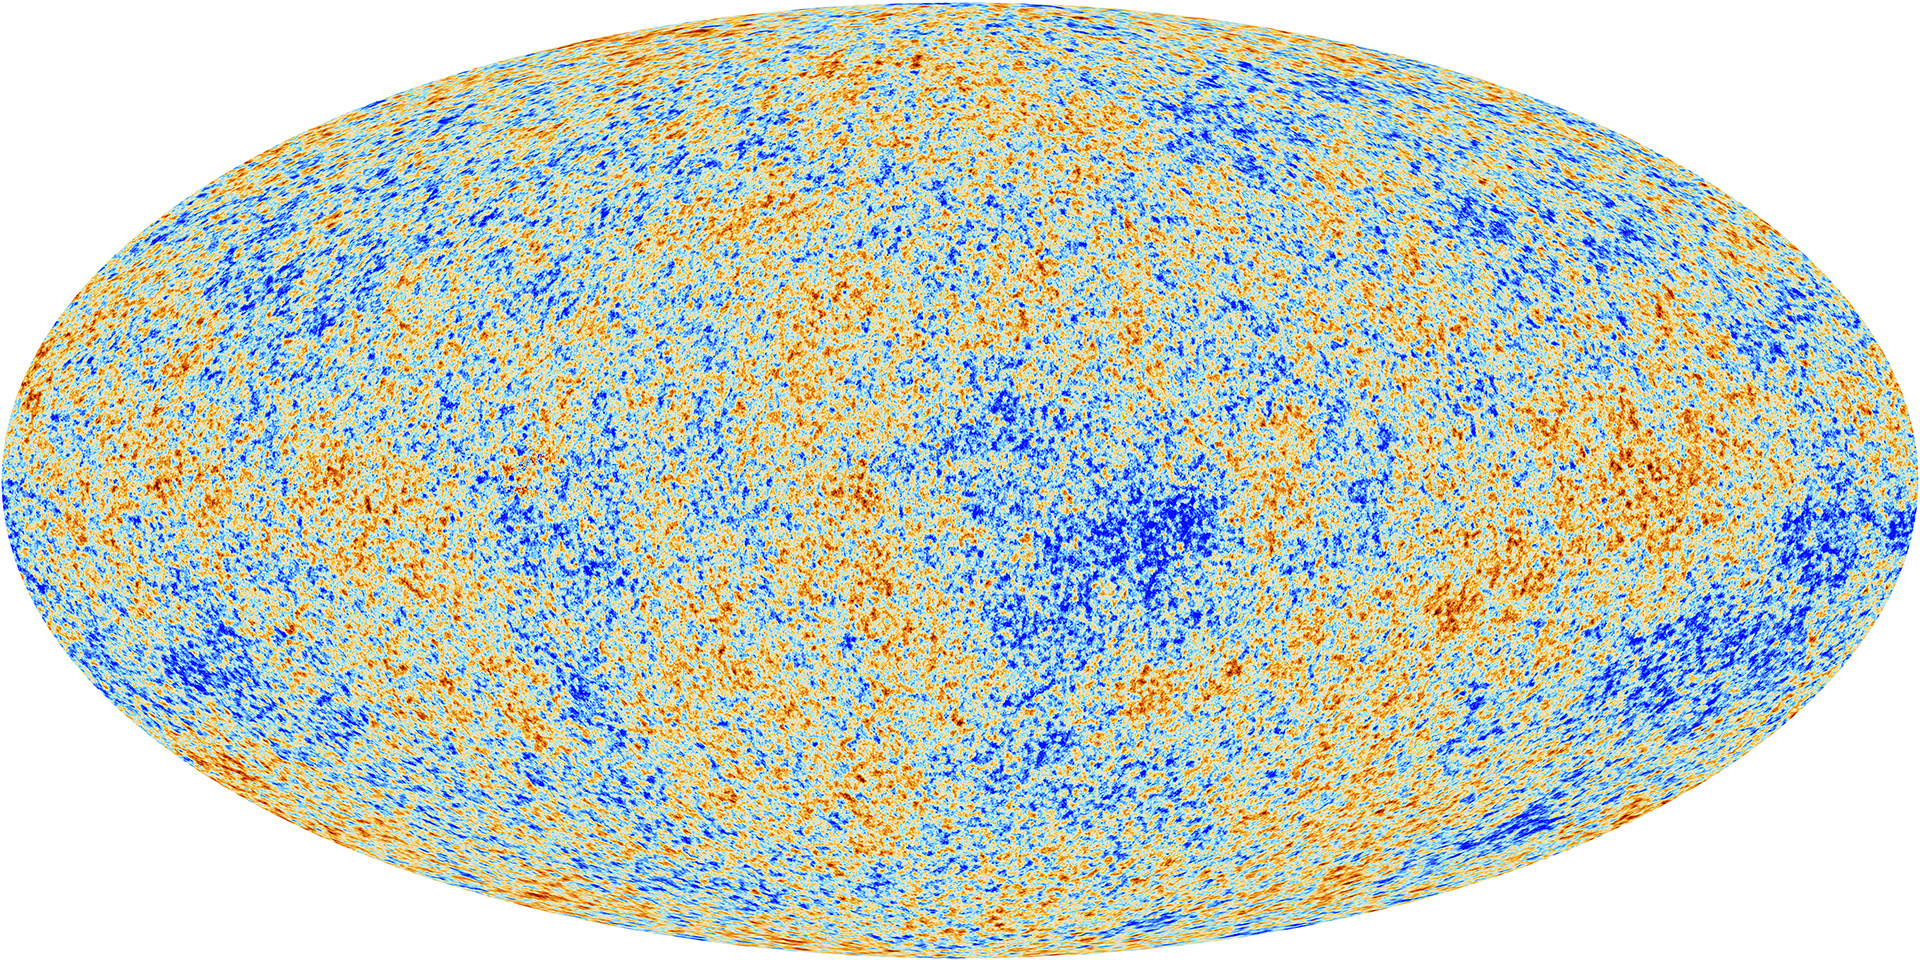
\includegraphics[width=0.8\textwidth]{figures/Planck_CMB}
        %\caption{Carte de la température du fond diffus cosmologique. La couleur indique 
        %les déviation de la température du corps noir. Ces déviations sont extrêmements petites, 
%supportant l'argument que l'Univers est localement isotropique. Crédit: \textit{ESA and the Planck Collaboration}.}
        %\label{fig:}
%\end{figure}

%L'homogénéité encode le fait que la métrique qui décrit l'espace-temps doit être la même 
%peut importe l'endroit dans l'Univers où l'observateur se situe. C'est une affirmation qui 
%concerne la distribution de matière et d'énergie dans l'Univers. Un Univers est homogène dans 
%le sens où la distribution de la matière et d'énergie est elle aussi homogène. Ainsi, 
%par les équations de champs d'Einstein qui relient le tenseur d'énergie-impulsion 
%à la courbure de l'espace-temps, on peut voir comment une affirmation qui concerne 
%la métrique implique immédiatement certaines propriétés pour la matière:
%\begin{equation}\label{eq:EFE}
        %G_{\mu\nu} = \frac{8 \pi G}{c^{4}} T_{\mu \nu}
%\end{equation} 
%Une étude de la distribution des galaxies dans l'Univers proche renforce se point, où 
%on remarque que la distribution de galaxies à l'intérieurs de sphères plus grande que 
%$r = 40\, \mathrm{Mpc}$ est étonnamment homogène. Gaussian distribution.

%metrique FLRW
%assume univers plat (k=0)
%distance comobile -> ell
%redshift
%distance angulaire
%\begin{figure}[H]
        %\centering
        %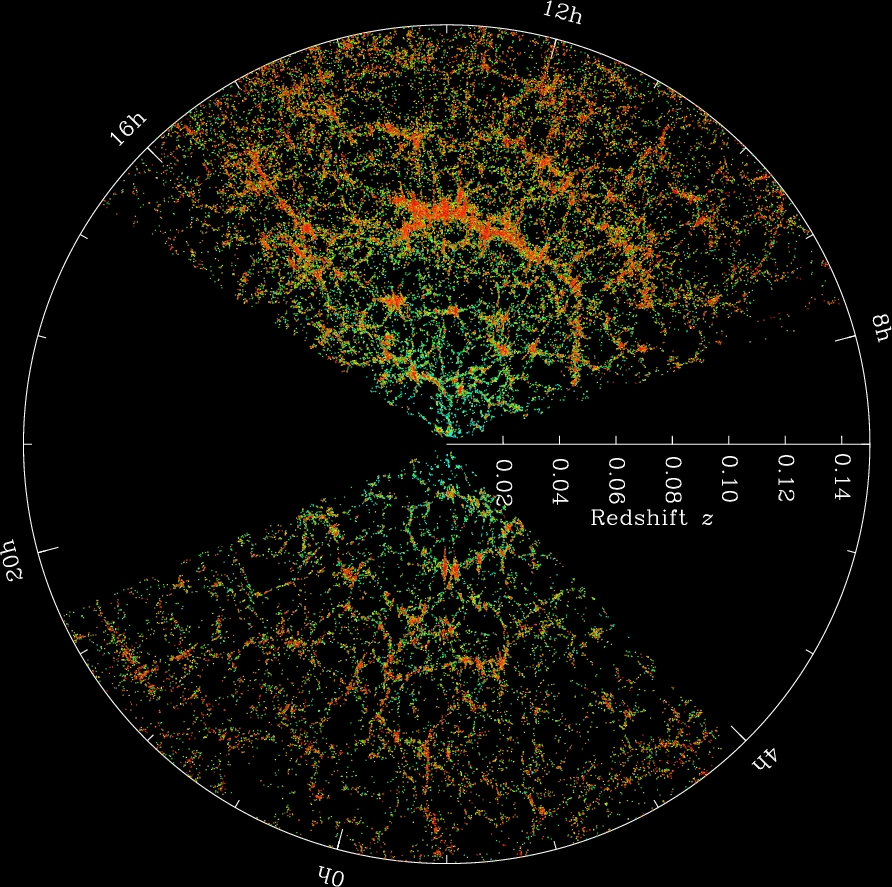
\includegraphics[width=\textwidth]{figures/sdss_universe}
        %\caption{Carte des galaxies prise par le Sloan Digital Sky Survey telescope montrant 
        %le niveau d'homogénéité et d'isotropie de l'Univers local. Chaque point est 
        %coloré par le niveau de densité local.}
        %\label{fig:sdss}
%\end{figure}


%Les symmétries encode une métrique qui est maximalement symmétrique au niveau spatial. On encode 
%l'évolution spatiale avec la facteur $a(t)$. On doit encore régler la question de la courbue de 
%l'espace. En fait, les symmétries du principe cosmologique sont agnostiques sur cette question, 
%de sorte qu'on doit encore faire un postulat.


